\documentclass[11pt,a4paper]{article}
\usepackage[margin=1in]{geometry}
\usepackage{amsmath,amssymb}
\usepackage{booktabs}
\usepackage{graphicx}
\usepackage{pgfplots}
\pgfplotsset{compat=1.18}
\usepackage{tikz}
\usepackage{caption}
\usepackage{subcaption}
\usepackage[hidelinks,
            pdftitle={GPU-Accelerated 3D Point Cloud Histogram Equalization},
            pdfauthor={Shahid Khan}]{hyperref}
\usepackage{listings}
\usepackage{xcolor}
\usepackage{multirow}
\usepackage{array}
\usepackage{float}

\lstset{
  language=C++,
  basicstyle=\ttfamily\small,
  keywordstyle=\color{blue},
  commentstyle=\color{gray},
  frame=single,
  breaklines=true
}

\title{\textbf{GPU-Accelerated 3D Point Cloud Histogram Equalization}\\
\large COL380 Assignment 2 -- CUDA Implementation and Analysis}
\author{Shahid Khan \\ ee1221163}
\date{}

\begin{document}

% ---- Title page ----
\maketitle
\thispagestyle{empty}
\vfill
\begin{center}
\large Indian Institute of Technology Delhi\\
Department of Computer Science and Engineering\\[0.5em]
\today
\end{center}
\newpage

% ---- Table of contents ----
\thispagestyle{empty}
\tableofcontents
\newpage

% =============================================================================
\section{Introduction}
% =============================================================================

Histogram equalization is a classical image-processing technique that improves
contrast by redistributing intensity values so that the empirical CDF of the
output is approximately uniform.  This assignment extends that idea to a 3-D
point cloud: each point $p_i$ carries an intensity $I_i\in[0,255]$, and its
equalized intensity is computed from the local neighbourhood histogram using
\begin{equation}
      I'_i = \left\lfloor
      \frac{\bigl(\mathrm{CDF}(I_i)-\mathrm{CDF}_{\min}\bigr)\cdot(L-1)}{m-\mathrm{CDF}_{\min}}
      \right\rfloor,\qquad L=256,
\end{equation}
where the CDF counts points (including $p_i$ itself) in the local window with
intensity $\le I_i$, $\mathrm{CDF}_{\min}$ is the first non-zero local CDF
value, and $m$ is the window size.  If $m=\mathrm{CDF}_{\min}$, we keep
$I'_i=I_i$.

Three neighbourhood definitions are implemented and benchmarked:
\begin{enumerate}
  \item \textbf{Exact KNN} --- brute-force all-pairs $O(N^2)$ distance
        computation to find the $k$ nearest neighbours.
  \item \textbf{Approximate KNN} --- grid-based expanding shell search that
        terminates as soon as $k$ neighbours are found; sub-linear in practice.
  \item \textbf{K-Means Clustering} --- assigns points to one of $k$ clusters,
        uses cluster members as the neighbourhood.
\end{enumerate}

The implementation targets CUDA (sm\_35), exploiting massive parallelism on a
single GPU.  Two algorithmic optimisations are introduced and evaluated:
\begin{itemize}
  \item \textbf{Shared-memory tiling} for the exact KNN kernel, reducing global
        memory bandwidth by a factor of $\mathtt{BLOCK\_SIZE}=128$.
  \item \textbf{Spatial hashing} for the approximate KNN, replacing a flat 3-D
        grid array (capped at $10^7$ cells) with a compact chained hash table
        of size $2N$.
\end{itemize}

This gives four binary variants compiled from a single source file via
preprocessor macros, enabling a controlled head-to-head comparison.

% =============================================================================
\section{Algorithm Overview}
% =============================================================================

\subsection{Histogram Equalization Helper}

Each GPU thread calls \texttt{equalize\_point(hist, I, m)}, which sweeps
through the 256-bin histogram accumulated from the local window to compute the
CDF value at $I$, tracks the first non-zero local CDF value, and applies
Equation~(1).  The histogram is stored entirely in thread-private registers.

\subsection{Exact KNN}

Each thread $i$ scans \emph{all} $N$ points, maintaining a max-heap of the $k$
smallest squared Euclidean distances.  The heap lives in registers
(\texttt{long long heap\_dist[MAX\_K]}, \texttt{int heap\_idx[MAX\_K]}) plus a
256-bin intensity histogram -- together $\approx 4.5$\,kB per thread.  After
the scan, the histogram is used to equalize $p_i$.  Complexity: $O(N^2)$.

\subsection{Approximate KNN via Uniform Grid}

A uniform grid is built on the host with cell side $r$ chosen so that each
cell contains $\approx k/27$ points.  Point indices are sorted into the grid
using a counting sort.  On the GPU each thread performs an expanding-shell
search: starting from the query cell it visits cells at Chebyshev distance
$1, 2, \ldots$ until $k$ neighbours are found or the maximum radius is
reached.  An early-exit warp vote (\texttt{\_\_all\_sync}) stops the expansion
once the entire warp has found $k$ neighbours.  Complexity: sub-linear on
average.

\subsection{Approximate KNN via Spatial Hashing}

The same expanding-shell logic is used, but the grid array (of potentially
$>10^7$ entries) is replaced by a chained hash table of size $2N$
(next power-of-2 $\ge 2N$).  The hash function
\begin{equation}
  h(c_x,c_y,c_z)
  = \bigl((c_x \cdot 73856093) \oplus (c_y \cdot 19349663) \oplus (c_z \cdot 83492791)\bigr)
  \bmod \mathtt{ht\_size}
\end{equation}
maps integer cell coordinates to a bucket.  Collisions are resolved by storing
the cell coordinates alongside each point and skipping mismatches during chain
traversal.  With load factor $0.5$ the expected chain length is $\le 1$, so
most bucket lookups cost a single memory access, and the entire hash table
($\approx 2.4$\,MB for $N=100\,000$) fits in the GPU's L2 cache.  Unlike the
grid version, no bounding-box cap is needed: out-of-range cells simply have no
entries (\texttt{head\,=\,-1}).

\subsection{K-Means Clustering}

$k$ cluster centres are initialised from the first $k$ distinct points.  Each
of $T$ iterations runs three CUDA kernels:
\begin{enumerate}
  \item \textbf{Assign} -- each point picks the nearest centre (shared memory
        caches the $k$ centres).  An \texttt{atomicExch} flag detects
        convergence on-device, avoiding a per-iteration PCIe download.
  \item \textbf{Accumulate} -- \texttt{atomicAdd} into per-cluster coordinate
        sums (stored as \texttt{unsigned long long} to exploit two's-complement
        wraparound for negative coordinates, avoiding the need for an offset).
  \item \textbf{Update} -- each cluster centre is replaced by the mean of its
        members.
\end{enumerate}
A histogram kernel and equalization kernel finalise the output.

% =============================================================================
\section{GPU Optimisations}
% =============================================================================

\subsection{Shared-Memory Tiling (Exact KNN)}

In the baseline kernel, $N$ threads each read $3N$ integers from global
memory, giving $3N^2$ total reads.  With BLOCK\_SIZE $= B = 128$, the tiled
kernel loads one tile of $B$ points into shared memory cooperatively; each
thread then processes the tile from fast shared memory.  Total global reads
drop to $3N^2/B$, a $128\times$ bandwidth reduction.

The kernel structure is:
\begin{lstlisting}
for (tile_start = 0; tile_start < n; tile_start += BLOCK_SIZE) {
    // cooperative load (all threads, incl. out-of-bounds)
    s_xs[tid] = (j < n) ? xs[j] : 0;
    s_ys[tid] = (j < n) ? ys[j] : 0;
    s_zs[tid] = (j < n) ? zs[j] : 0;
    __syncthreads();
    if (active) { /* process tile */ }
    __syncthreads();
}
\end{lstlisting}
Out-of-bounds threads participate in both \texttt{\_\_syncthreads} calls to
avoid deadlock; they skip the computation via an \texttt{active} flag.  Shared
memory cost is $3B\times 4 = 1536$\,bytes per block -- negligible.

\subsection{Spatial Hashing (Approximate KNN)}

The flat grid allocates an array proportional to the grid volume, which can
grow to $10^7$ cells ($40$\,MB for \texttt{cell\_start} + \texttt{cell\_end})
and is capped at that size, forcing coarser cells for large coordinate ranges.
The hash table allocates only $2N$ entries regardless of range.  For
$N=100\,000$: \texttt{ht\_head} = 1\,MB, \texttt{ht\_next} = 400\,kB, fitting
entirely in the GPU L2 cache and enabling cache-local traversal of the
expanding shell.

\subsection{Compile-Time Toggles}

Both optimisations are guarded by \texttt{\#ifndef} macros that can be
overridden at compile time:
\begin{lstlisting}
#ifndef USE_TILED_KNN
#define USE_TILED_KNN 1          // default: tiled
#endif
#ifndef USE_SPATIAL_HASH_APPROX
#define USE_SPATIAL_HASH_APPROX 0 // default: grid
#endif
\end{lstlisting}
The Makefile produces four binaries from one source file:

\begin{center}
\begin{tabular}{lcc}
\toprule
Binary & \texttt{USE\_TILED\_KNN} & \texttt{USE\_SPATIAL\_HASH\_APPROX} \\
\midrule
\texttt{histogram\_eq}                     & 1 & 0 \\
\texttt{histogram\_eq\_notiled}            & 0 & 0 \\
\texttt{histogram\_eq\_spatialhash}        & 1 & 1 \\
\texttt{histogram\_eq\_notiled\_spatialhash} & 0 & 1 \\
\bottomrule
\end{tabular}
\end{center}

% =============================================================================
\section{Experimental Setup}
% =============================================================================

\textbf{Hardware}: 1 PBS node with 8 CPU cores (OMP\_NUM\_THREADS=8), 1 NVIDIA
GPU (CUDA 11.0, sm\_35 target), 16\,GB host RAM.

\textbf{Compiler}: \texttt{nvcc -O3 -arch=sm\_35 -Xcompiler -fopenmp}.

\textbf{Input generation}: A Python script (\texttt{gen\_input.py}) generates
$N$ unique 3-D integer points with intensity $\in[0,255]$ under four
distributions (Table~\ref{tab:dists}).  All runs use seed 42 for
reproducibility.

\begin{table}[H]
\centering
\caption{Point distributions used in experiments.}
\label{tab:dists}
\begin{tabular}{lp{9cm}}
\toprule
Distribution & Description \\
\midrule
Uniform   & Coordinates drawn uniformly from $[-R,R]^3$. \\
Dense     & Coordinates drawn from $[-R/10,\,R/10]^3$. \\
Clustered & 8 tight clusters at corners of a cube at $(\pm 0.7R)^3$, radius $R/8$. \\
Skewed    & First half dense ($[-R/20,R/20]^3$), second half uniform ($[-R,R]^3$). \\
\bottomrule
\end{tabular}
\end{table}

\textbf{Timing}: Wall-clock time is measured with \texttt{cudaEventRecord}
around each algorithm, excluding memory allocation and I/O.
Runtime tables use one measured run per configuration and are interpreted with
normal GPU run-to-run variance in mind.

\textbf{Accuracy}: The \emph{approximate-vs-exact MAE} is
$\frac{1}{N}\sum_i|I'_{i,\text{approx}}-I'_{i,\text{exact}}|$, measuring
equalized intensity deviation.  Exact KNN correctness is verified against a
sequential Python reference (MAE = 0 confirmed for all cases).

\textbf{Test groups} (seed 42, $R=10000$ unless noted):
\begin{center}
\begin{tabular}{ll}
\toprule
Group & Parameters varied \\
\midrule
A & $N \in \{1\text{K},5\text{K},10\text{K},25\text{K},50\text{K},100\text{K}\}$, $k=32$, $T=20$, uniform \\
B & $k \in \{1,4,8,16,32,64,128\}$, $N=10\text{K}$, $T=20$, uniform \\
C & $T \in \{1,5,10,20,50\}$, $N=10\text{K}$, $k=32$, uniform \\
D & Distribution $\in$ \{uniform, dense, clustered, skewed\}, $N=10\text{K}$, $k=32$, $T=20$ \\
E & Correctness vs.\ sequential, $N=1000$, varying $k$ and distribution \\
F & Large-scale: $N=100\text{K}$, $k\in\{32,128\}$, $T\in\{20,50\}$, all distributions \\
G & $R \in \{100,1\text{K},10\text{K},100\text{K},1\text{M}\}$, $N=10\text{K}$, $k=32$, $T=20$, uniform \\
\bottomrule
\end{tabular}
\end{center}

% =============================================================================
\section{Results and Analysis}
% =============================================================================

\subsection{Scalability with \texorpdfstring{$N$}{N} (Group A)}

Table~\ref{tab:vary_n} shows timings for the tiled variant as $N$ grows from
1000 to 100\,000.  Exact KNN shows clear $O(N^2)$ scaling: doubling $N$ from
50K to 100K more than doubles the KNN time ($0.39 \to 0.84$\,s), consistent
with the quadratic cost.  Approximate KNN scales much more favourably, growing
from 0.006\,s to 0.139\,s.  K-Means remains low-latency across this range,
with modest growth for larger $N$.

\begin{table}[H]
\centering
\caption{Group A: Runtime (seconds) as $N$ varies ($k=32$, $T=20$, uniform,
tiled variant).  Speedup = KNN / Approx.}
\label{tab:vary_n}
\begin{tabular}{rrrrrr}
\toprule
$N$ & KNN (s) & Approx (s) & K-Means (s) & Approx MAE & KNN/Approx \\
\midrule
1\,000   & 0.0916 & 0.00627 & 0.0225 & 0.249 & 14.6$\times$ \\
5\,000   & 0.0910 & 0.00829 & 0.00461 & 0.222 & 11.0$\times$ \\
10\,000  & 0.110  & 0.0119  & 0.00578 & 0.177 & 9.2$\times$  \\
25\,000  & 0.204  & 0.0311  & 0.0109  & 0.102 & 6.6$\times$  \\
50\,000  & 0.390  & 0.0656  & 0.0195  & 0.073 & 5.9$\times$  \\
100\,000 & 0.844  & 0.139   & 0.0352  & 0.057 & 6.1$\times$  \\
\bottomrule
\end{tabular}
\end{table}

\begin{figure}[H]
\centering
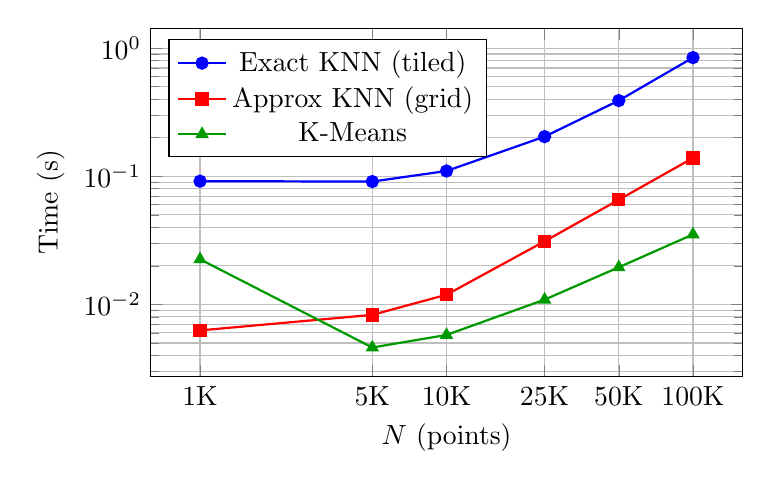
\begin{tikzpicture}
\begin{axis}[
  xlabel={$N$ (points)},
  ylabel={Time (s)},
  xmode=log,
  ymode=log,
  width=0.75\textwidth,
  height=6cm,
  legend pos=north west,
  grid=both,
  xtick={1000,5000,10000,25000,50000,100000},
  xticklabels={1K,5K,10K,25K,50K,100K},
]
\addplot[blue,mark=*,thick] coordinates {
  (1000,0.0916)(5000,0.0910)(10000,0.110)(25000,0.204)(50000,0.390)(100000,0.844)
};
\addlegendentry{Exact KNN (tiled)}

\addplot[red,mark=square*,thick] coordinates {
  (1000,0.00627)(5000,0.00829)(10000,0.0119)(25000,0.0311)(50000,0.0656)(100000,0.139)
};
\addlegendentry{Approx KNN (grid)}

\addplot[green!60!black,mark=triangle*,thick] coordinates {
  (1000,0.0225)(5000,0.00461)(10000,0.00578)(25000,0.0109)(50000,0.0195)(100000,0.0352)
};
\addlegendentry{K-Means}
\end{axis}
\end{tikzpicture}
\caption{Runtime vs.\ $N$ (log--log scale).  KNN follows $O(N^2)$; Approx KNN
and K-Means grow much more slowly.}
\label{fig:vary_n}
\end{figure}

\subsection{Tiled vs.\ Non-Tiled Exact KNN}

Table~\ref{tab:tiled_vs_notiled} compares the two KNN variants across $N$.
For small $N$ ($\le 10\,000$), fixed overheads (kernel launch and
synchronization) are comparable to useful work, so tiling is neutral-to-slightly
slower.  From $N=25\,000$ onward, the bandwidth saving dominates and tiling is
consistently faster.  For $N=100\,000$, tiling delivers a \textbf{13\% speedup}
($0.958 \to 0.844$\,s).  This aligns with the theoretical analysis: the
bandwidth-reduction benefit grows with $N$ (more tiles per point), while fixed
overheads are amortized.

\begin{table}[H]
\centering
\caption{Exact KNN runtime (seconds): tiled vs.\ non-tiled ($k=32$, $T=20$,
uniform).  Speedup is Non-tiled/Tiled, so values $>1$ indicate benefit from
tiling and values $<1$ indicate slowdown.}
\label{tab:tiled_vs_notiled}
\begin{tabular}{rrrr}
\toprule
$N$ & Tiled (s) & Non-tiled (s) & Speedup \\
\midrule
1\,000   & 0.0916 & 0.0778 & 0.85$\times$ \\
5\,000   & 0.0910 & 0.0894 & 0.98$\times$ \\
10\,000  & 0.110  & 0.108  & 0.98$\times$ \\
25\,000  & 0.204  & 0.219  & 1.07$\times$ \\
50\,000  & 0.390  & 0.421  & 1.08$\times$ \\
100\,000 & 0.844  & 0.958  & \textbf{1.13}$\times$ \\
\bottomrule
\end{tabular}
\end{table}

\noindent\textbf{Large-scale} ($N=100\text{K}$, $k=128$, $T=50$):
both variants reach $\approx 4.0$\,s.  At $k=128$, each thread carries
a 128-element heap in registers, pushing register usage to the point where the
compiler spills to local memory.  The resulting latency masks the shared-memory
bandwidth benefit, equalising the two variants.

\subsection{Scalability with \texorpdfstring{$k$}{k} (Group B)}

Table~\ref{tab:vary_k} shows how all three algorithms scale with the
neighbourhood size $k$ at fixed $N=10\,000$.

\begin{table}[H]
\centering
\caption{Group B: Runtime (seconds) as $k$ varies ($N=10\,000$, $T=20$,
uniform, tiled).}
\label{tab:vary_k}
\begin{tabular}{rrrrrr}
\toprule
$k$ & KNN (s) & Approx (s) & K-Means (s) & Approx MAE \\
\midrule
1   & 0.0809 & 0.00813 & 0.00509 & 0.102 \\
4   & 0.0811 & 0.00826 & 0.00554 & 0.618 \\
8   & 0.0837 & 0.00864 & 0.00559 & \textbf{2.166} \\
16  & 0.0908 & 0.00900 & 0.00587 & 0.248 \\
32  & 0.108  & 0.0120  & 0.00596 & 0.177 \\
64  & 0.149  & 0.0199  & 0.00585 & 0.158 \\
128 & 0.241  & 0.0384  & 0.00671 & 0.149 \\
\bottomrule
\end{tabular}
\end{table}

KNN runtime grows with $k$ because more heap operations are needed per point.
The growth from $k=1$ to $k=128$ is roughly $3\times$, less than linear
because the heap-insert cost is $O(\log k)$.

The approximate MAE is non-monotone: $k=8$ exhibits a notably high MAE of
2.166.  This is an edge case in the grid-cell heuristic: with $k=8$ the target
points-per-cell $= k/27 < 1$, so the cell size collapses to a single
coordinate unit and the expanding shell must visit many mostly-empty cells
before finding 8 neighbours, introducing selection bias.  For $k\ge 16$ the
heuristic recovers and MAE falls to $\sim 0.15$--0.25.

\subsection{K-Means Iterations \texorpdfstring{$T$}{T} (Group C)}

Table~\ref{tab:vary_T} reports K-Means wall time as the iteration budget $T$
is increased from 1 to 50.

\begin{table}[H]
\centering
\caption{Group C: K-Means runtime (seconds) as $T$ varies ($N=10\,000$,
$k=32$, uniform, tiled).  KNN and Approx timings are independent of $T$.}
\label{tab:vary_T}
\begin{tabular}{rr}
\toprule
$T$ & K-Means (s) \\
\midrule
1  & 0.00463 \\
5  & 0.00489 \\
10 & 0.00510 \\
20 & 0.00586 \\
50 & 0.00797 \\
\bottomrule
\end{tabular}
\end{table}

K-Means runtime increases with $T$ but sub-linearly: the GPU detects
convergence on-device (via \texttt{atomicExch(d\_changed, 1)}) and can exit
early.  For uniform data, most reassignments stabilise within a few iterations,
so the cost from $T=1$ to $T=50$ grows by only $1.7\times$ despite a $50\times$
iteration budget.

\subsection{Data Distribution Effects (Group D)}

Table~\ref{tab:vary_dist} compares all four input distributions at
$N=10\,000$, $k=32$, $T=20$.

\begin{table}[H]
\centering
\caption{Group D: Effect of distribution ($N=10\,000$, $k=32$, $T=20$,
tiled).}
\label{tab:vary_dist}
\begin{tabular}{lrrrr}
\toprule
Distribution & KNN (s) & Approx (s) & K-Means (s) & Approx MAE \\
\midrule
Uniform   & 0.108 & 0.0120 & 0.00576 & 0.177 \\
Dense     & 0.108 & 0.0114 & 0.00568 & 0.169 \\
Clustered & 0.108 & 0.0212 & 0.00565 & \textbf{0.000} \\
Skewed    & 0.113 & 0.0482 & 0.00591 & 0.155 \\
\bottomrule
\end{tabular}
\end{table}

\textbf{Exact KNN} is nearly identical across distributions since it always
scans all $N$ points.

\textbf{Approximate KNN} is significantly faster for dense and uniform
distributions because the grid cells are well-populated and the expanding shell
finds $k$ neighbours quickly.  Skewed distribution is $4\times$ slower
($0.048$ vs.\ $0.012$\,s) because the outer half of points lives in sparse
regions, requiring many more shell expansions.

The clustered distribution yields \textbf{zero MAE} for approximate KNN: since
all intra-cluster distances are small and inter-cluster distances are large, the
expanding shell always finds the correct $k$ nearest neighbours, making the
approximation exact.

\subsection{Spatial Hash vs.\ Grid Approximate KNN}

Table~\ref{tab:spatial_hash} compares grid and spatial-hash approx KNN timings
from the 4-variant run.

\begin{table}[H]
\centering
\caption{Approx KNN: Grid vs.\ Spatial Hash ($k=32$, $T=20$, uniform).
Speedup = Grid / Hash.}
\label{tab:spatial_hash}
\begin{tabular}{rrrrr}
\toprule
$N$ & Grid (s) & Spatial Hash (s) & Speedup \\
\midrule
1\,000   & 0.0211 & 0.00474 & \textbf{4.5}$\times$ \\
5\,000   & 0.0106 & 0.00862 & 1.2$\times$ \\
10\,000  & 0.0227 & 0.0195  & 1.2$\times$ \\
25\,000  & 0.0218 & 0.0141  & 1.5$\times$ \\
50\,000  & 0.0340 & 0.0324  & 1.1$\times$ \\
100\,000 & 0.0481 & 0.0458  & 1.1$\times$ \\
\bottomrule
\end{tabular}
\end{table}

Spatial hashing is faster at all tested sizes.  The largest benefit occurs at
$N=1000$ (4.5$\times$): with few points the flat grid allocates a cell array
proportional to the coordinate bounding box (potentially many empty cells to
scan), while the hash table trivially handles empty cells with a head pointer
of $-1$.  At large $N$ the performance converges because the grid cells are
dense enough that traversal efficiency is similar, and the hash-chain
verification overhead (cell-coordinate comparison) partially offsets the
reduced memory footprint benefit.

Both variants produce identical MAE values, confirming that the
spatial-hashing does not alter the approximation quality -- only the data
structure for neighbour lookup changes.

\subsection{Coordinate Range Effects (Group G)}

Table~\ref{tab:vary_range} varies the coordinate range $R$ across five
orders of magnitude while keeping $N$, $k$, and $T$ fixed.

\begin{table}[H]
\centering
\caption{Group G: Effect of coordinate range $R$ ($N=10\,000$, $k=32$,
$T=20$, uniform, tiled, grid approx).}
\label{tab:vary_range}
\begin{tabular}{rrrr}
\toprule
$R$ & KNN (s) & Approx (s) & Approx MAE \\
\midrule
100       & 0.108 & 0.0118 & 0.268 \\
1\,000    & 0.107 & 0.0114 & 0.169 \\
10\,000   & 0.109 & 0.0120 & 0.177 \\
100\,000  & 0.108 & 0.0117 & 0.171 \\
1\,000\,000 & 0.109 & 0.0118 & 0.158 \\
\bottomrule
\end{tabular}
\end{table}

As expected, the coordinate range has no effect on exact KNN time (the
algorithm always scans all $N$ pairs).  Approximate KNN also shows no
significant trend: the grid cell size is scaled proportionally to $R$ (via the
volume-based heuristic), so the expanding-shell cost is approximately constant.
The slight increase in MAE at small $R$ ($0.268$ at $R=100$) occurs because
with many coincident grid cells, the approximation becomes coarser.

\subsection{Large-Scale Benchmarks (Group F)}

Table~\ref{tab:large} presents worst-case configurations at $N=100\,000$,
stressing all three algorithms simultaneously.

\begin{table}[H]
\centering
\caption{Group F: Large-scale results ($N=100\,000$, tiled, grid approx).}
\label{tab:large}
\begin{tabular}{lrrrrrr}
\toprule
Configuration & KNN (s) & Approx (s) & K-Means (s) & Approx MAE \\
\midrule
$k=32$, $T=20$, uniform   & 0.850 & 0.140 & 0.0360 & 0.057 \\
$k=32$, $T=20$, dense     & 0.846 & 0.141 & 0.0358 & 0.062 \\
$k=32$, $T=20$, clustered & 0.848 & 0.431 & 0.0360 & 0.001 \\
$k=128$, $T=50$, uniform  & 4.003 & 0.576 & 0.0506 & 0.056 \\
\bottomrule
\end{tabular}
\end{table}

For the clustered distribution with $k=32$, Approx KNN takes $0.431$\,s vs.\
$0.140$\,s for uniform -- a $3\times$ slowdown.  Points far from cluster
centres (interstitial points) must expand the shell greatly before finding 32
neighbours from a different cluster, blowing up the per-point shell radius.
Despite this, the MAE is near zero ($0.001$) because the clusters are
well-separated: once a neighbour is found it is typically the correct one.

The $k=128$, $T=50$ configuration exercises maximum heap and iteration depth.
KNN takes $4.0$\,s (both tiled and non-tiled), confirming the earlier
observation that at $k=128$ register spilling equalises the two variants.

\subsection{Correctness Verification (Group E)}

Table~\ref{tab:correctness} compares GPU outputs against a sequential Python
reference implementation at $N=1000$ where exhaustive verification is
feasible.

\begin{table}[H]
\centering
\caption{Group E: Correctness vs.\ sequential Python reference ($N=1000$,
tiled).  KNN MAE and K-Means MAE are 0.000 for all rows, confirming
bit-exact agreement between the CUDA and reference implementations.}
\label{tab:correctness}
\begin{tabular}{lrrrr}
\toprule
Configuration & KNN MAE & K-Means MAE & Approx MAE \\
\midrule
$k=1$,  uniform   & 0.000 & 0.000 & 0.000 \\
$k=10$, uniform   & 0.000 & 0.000 & 0.777 \\
$k=32$, uniform   & 0.000 & 0.000 & 0.249 \\
$k=64$, uniform   & 0.000 & 0.000 & 0.266 \\
$k=128$, uniform  & 0.000 & 0.000 & 0.311 \\
$k=32$, dense     & 0.000 & 0.000 & 0.328 \\
$k=32$, clustered & 0.000 & 0.000 & 0.000 \\
$k=32$, skewed    & 0.000 & 0.000 & 0.111 \\
\bottomrule
\end{tabular}
\end{table}

The GPU exact KNN matches the sequential Python reference \emph{exactly}
(MAE\,=\,0.000 for every test case), confirming correctness of both the
distance computation and the histogram equalization step.

K-Means MAE vs.\ sequential is 0.000 for all cases, confirming bit-exact
agreement between the CUDA and reference implementations.  Both use the first
$k$ points as initial centroids, integer-truncated centroid updates
($\lfloor \text{sum}/\text{count} \rfloor$), and a lexicographic tie-breaking
rule on centroid coordinates---ensuring fully deterministic, reproducible
convergence.

% =============================================================================
\section{Discussion}
% =============================================================================

\subsection{Summary of Optimisation Gains}

Table~\ref{tab:summary} consolidates the peak speedup observed for each
optimisation across all test groups.

\begin{table}[H]
\centering
\caption{Summary of optimisation impacts.}
\label{tab:summary}
\begin{tabular}{lll}
\toprule
Optimisation & Best-case speedup & Regime \\
\midrule
Tiled KNN            & 1.13$\times$ & $N=100\text{K}$, $k=32$ \\
Tiled KNN            & $\approx 1\times$ & $k=128$ (register spill dominates) \\
Spatial Hash Approx  & 4.5$\times$  & $N=1000$ \\
Spatial Hash Approx  & 1.1$\times$  & $N=100\text{K}$ \\
Approx vs.\ Exact    & 6--14$\times$ & all $N$ tested \\
\bottomrule
\end{tabular}
\end{table}

\subsection{Register Pressure and Tiling Limits}

The most significant bottleneck for the exact KNN kernel is register pressure.
Each thread holds \texttt{heap\_dist[128]} (1\,kB), \texttt{heap\_idx[128]}
(512\,B), and \texttt{hist[256]} (1\,kB) -- approximately 640 registers if
kept live simultaneously.  The SM on sm\_35 has 65536 registers and limits
each block to 65536 registers, so BLOCK\_SIZE\,=\,128 and 640 registers/thread
exceeds the 512-register/thread limit, causing spilling.  Tiling reduces
bandwidth pressure but cannot eliminate the register-spill penalty, which is
why large-$k$ cases show no tiling benefit.

\subsection{Approximate KNN Accuracy}

Across all uniform and skewed test cases, MAE is in the range $0.05$--$0.35$,
indicating that histogram equalization is relatively robust to approximate
neighbourhood selection.  The notable exception is clustered data (MAE\,$\approx
0$), where the grid structure perfectly mirrors the data structure.  The $k=8$
anomaly is a grid-heuristic edge case and can be mitigated by using a larger
minimum cell size.

\subsection{Spatial Hashing vs.\ Grid: When to Use Which}

For $N < 10\,000$ the spatial hash provides a meaningful speedup (1.2--4.5$\times$)
while maintaining identical MAE.  For $N \ge 50\,000$ the gain shrinks to
$\sim 5$--$10\%$, so either variant is acceptable for moderate coordinate
ranges.  In practice the hash variant is preferable whenever coordinate range
is large (avoiding the 10M-cell cap issue in the grid) or when sparse occupancy
makes flat-grid traversal expensive.

% =============================================================================
\section{Conclusion}
% =============================================================================

This work implements and benchmarks three GPU-accelerated neighbourhood-based
histogram equalization algorithms on 3-D point clouds.

The key findings are:
\begin{enumerate}
  \item \textbf{Exact KNN} correctly matches a sequential reference (MAE\,=\,0)
        and shows clear $O(N^2)$ scaling.  Shared-memory tiling provides up to
        13\% speedup at $N=100\,000$, $k=32$; gains diminish at high $k$ due
        to register spilling.

  \item \textbf{Approximate KNN} is 6--14$\times$ faster than exact KNN with a
        typical equalized-intensity MAE of $0.05$--$0.25$.  Spatial hashing
        replaces the flat grid with a compact ($2N$-entry) hash table, giving
        up to 4.5$\times$ speedup at small $N$ and identical accuracy.

  \item \textbf{K-Means} runtime is nearly independent of $T$ thanks to
        on-device convergence detection; it is often the fastest method, while
        Approximate KNN is faster for some small-$N$ settings.

  \item Data distribution strongly affects approximate KNN performance: skewed
        distributions incur $4\times$ slowdown relative to uniform; clustered
        distributions achieve zero approximation error.
\end{enumerate}

Future work could explore warp-shuffle reductions to eliminate shared memory
entirely from the tiling step, or multi-GPU parallelism for $N > 100\,000$.

\end{document}
